% document type: science report
\documentclass[abstracton, a4paper, 12pt]{scrreprt}

% Encoding (utf8)
\usepackage[utf8]{inputenc}
\usepackage[T1]{fontenc}

% Silbentrennung (Neu-Deutsch)
\usepackage[ngerman]{babel}

% Literaturverzeichnis (Deutsch)
\usepackage{bibgerm}

% Farben
\usepackage{color}
\usepackage[table]{xcolor}
\definecolor{darkgreen}{rgb}{0,0.6,0}
\definecolor{darkgrey}{rgb}{0.5,0.5,0.5}
\definecolor{grey}{rgb}{0.8,0.8,0.8}
\definecolor{lightgrey}{rgb}{0.95,0.95,0.95}
\definecolor{mauve}{rgb}{0.58,0,0.82}

% Grafiken
\usepackage[pdftex]{graphicx}
\usepackage{epsfig}
% Umfliessen von Text um Tabellen und Bilder
\usepackage{wrapfig}

% Grafiken korrekt positionieren
\usepackage{float}
\restylefloat{figure}
\usepackage[section]{placeins}
\usepackage{subfigure}

% hyperlinks
\usepackage{hyperref}
\hypersetup{
   colorlinks,%
   citecolor=blue,%
   filecolor=blue,%
   linkcolor=blue,%
   urlcolor=blue
}
\urlstyle{same}

% Absatz
\setlength{\parindent}{0pt} % Absatzeinzug
\setlength{\parskip}{10pt} % Absatzabstand

% Glossar
\usepackage[toc]{glossaries}
\makeglossaries

% TODO Kommentare
\usepackage{todonotes}

% Definition vom Header und Footer im Seitenlayout
\usepackage{fancyhdr} 
\pagestyle{fancy} 
\fancyhf{}

% Linien nach dem Header und vor dem Footer
%\renewcommand{\footrulewidth}{0.4pt}
%\renewcommand{\headrulewidth}{0.4pt}

\fancyhead[L]{\footnotesize{\leftmark}}
\fancyfoot[C]{\footnotesize{\thepage}}
\fancyhead[R]{}

% Header auch bei Kapitelanfangsseite
\def\chapterpagestyle{fancy}

% Tabelle
% Padding links und rechts von Zelle
\setlength{\tabcolsep}{5px}
% Padding oben und unten (mittels arraystretch)
\renewcommand{\arraystretch}{1.3}

% Für schöne URLs
\usepackage{url}

% Syntaxhighlighter (benoetigt color und xcolor package)
\usepackage{listings}
 
\lstset{ %
  language=HTML,                % the language of the code
  basicstyle=\footnotesize,           % the size of the fonts that are used for the code
  numbers=left,                   % where to put the line-numbers
  numberstyle=\tiny\color{darkgrey},  % the style that is used for the line-numbers
  stepnumber=1,                   % the step between two line-numbers. If it's 1, each line will be numbered
  numbersep=5pt,                  % how far the line-numbers are from the code
  backgroundcolor=\color{white},  % choose the background color. You must add \usepackage{color}
  showspaces=false,               % show spaces adding particular underscores
  showstringspaces=false,         % underline spaces within strings
  showtabs=false,                 % show tabs within strings adding particular underscores
  frame=single,                   % adds a frame around the code
  rulecolor=\color{darkgrey},        % if not set, the frame-color may be changed on line-breaks within not-black text (e.g. commens (green here))
  tabsize=2,                      % sets default tabsize to 2 spaces
  captionpos=b,                   % sets the caption-position to bottom
  breaklines=true,                % sets automatic line breaking
  breakatwhitespace=false,        % sets if automatic breaks should only happen at whitespace
  title=\lstname,                   % show the filename of files included with \lstinputlisting;
                                  % also try caption instead of title
  keywordstyle=\color{blue},          % keyword style
  commentstyle=\color{darkgreen},       % comment style
  stringstyle=\color{mauve},         % string literal style
  escapeinside={\%*}{*)},            % if you want to add a comment within your code
  morekeywords={*,...}               % if you want to add more keywords to the set
}

% Javascript Syntaxhighliting
\lstdefinelanguage{JavaScript} {
	morekeywords={
		break,const,continue,delete,do,while,export,for,in,function,
		if,else,import,in,instanceOf,label,let,new,return,switch,this,
		throw,try,catch,typeof,var,void,with,yield
	},
	sensitive=false,
	morecomment=[l]{//},
	morecomment=[s]{/*}{*/},
	morestring=[b]",
	morestring=[d]'
}
\lstset{
	frame=tb,
	framesep=5pt,
	basicstyle=\footnotesize\ttfamily,
	showstringspaces=false,
	keywordstyle=\ttfamily\bfseries\color{blue},
	identifierstyle=\ttfamily,
	stringstyle=\ttfamily\color{mauve},
	commentstyle=\color{darkgreen},
	rulecolor=\color{darkgrey},
	xleftmargin=5pt,
	xrightmargin=5pt,
	aboveskip=\bigskipamount,
	belowskip=\bigskipamount
}

%% define toc formatting
%\usepackage[titles]{tocloft}
%\setlength{\cftsubsecindent}{3em}
%\setlength{\cftsubsecnumwidth}{3.3em}
%\setlength{\cftsubsubsecindent}{4.5em}
%\setlength{\cftsubsubsecnumwidth}{4em}

%% figure numbering
%\newcounter{myfigure}
%\renewcommand{\thefigure}{\arabic{myfigure}}
%\newcounter{mytable}
%\renewcommand{\thetable}{\arabic{mytable}}
%\usepackage{makeidx} \makeindex
%\makeglossary

%% Definition vom Seitenlayout
%\setlength{\topmargin}{-1.2cm}
%\setlength{\oddsidemargin}{0.5cm} 
%\setlength{\evensidemargin}{0.5cm}

%\setlength{\textheight}{24.5cm} 
%\setlength{\textwidth}{15cm}

%\setlength{\footskip}{1.2cm} 
%\setlength{\footnotesep}{0.4cm}

%% Neues Kapitel Makro, damit die Variablen korrekt abgefuellt werden
%\newcommand{\newchap}[1]{
%	\chapter{#1}
%	\markboth {Kapitel \thechapter.  {#1}}{Kapitel \thechapter.  {#1}}
%}
%
%% command to import a figure
%\newcommand{\fig}[5]{
%  \begin{figure}[h]
%    \begin{center}
%      \includegraphics[width=#4cm]{#1}
%    \end{center}
%    \stepcounter{myfigure}
%    \caption[#5]{#3}
%    \label{#2}
%  \end{figure}
%}
%
%\newcommand{\figtable}[4]{
%  \begin{figure}[h]
%    \begin{center}
%      {  
%			  \footnotesize
%  			\sffamily
%			  #3
%      }
%    \end{center}
%    \stepcounter{myfigure}
%    \caption[#4]{#2}
%    \label{#1}
%  \end{figure}
%}
%
%\newcommand{\tab}[4]{
%  \begin{table}[h]
%    \begin{center}
%      {  
%			  \footnotesize
%  			\sffamily
%  			\renewcommand{\arraystretch}{1.4}
%			  #3  			
%      }
%    \end{center}
%    \stepcounter{mytable}
%    \caption[#4]{#2}
%    \label{#1}
%  \end{table}
%}
%
%% command to refere to a figure
%\newcommand{\reffig}[1]{Abbildung \ref{#1}}
%
%% Definition des Nummerierungslevel
%\setcounter{secnumdepth}{4} 
%\setcounter{tocdepth}{4} 
%\setcounter{lofdepth}{1} 
%
%% Definition von Paragraphen
%\parskip=0.3cm
%\parindent=0cm
%
%% Definition vom Zeilenabstand
%\usepackage{setspace} % Zeilenabstand
%\onehalfspacing
%
%% Befehle fuer Anfuehrungszeichen
%\usepackage{xspace} % Leerschlag nach Anfuehrungszeichen
%\newcommand{\qr}{\grqq\xspace}
%\newcommand{\qrs}{\grqq\ }
%\newcommand{\ql}{\glqq}
%
%% Formatierungsbefehle zum Zitieren
%\newcommand{\page}[1]{S.~#1}
%\newcommand{\pagef}[1]{S.~#1f.}
%\newcommand{\pageff}[1]{S.~#1ff.}
%\newcommand{\pages}[2]{S.~#1--#2}

\begin{document}

% -----------------------------------------
% HEAD
% -----------------------------------------
% Titelseite
\title{Studienarbeit: Google Fusion Table Prototype}
\author{Jürg Hunziker\\jhunzike@hsr.ch
		\and
		Stefan Oderbolz\\soderbol@hsr.ch}
\date{29. Mai 2012}

\begin{titlepage}

% Logos

\includegraphics[width=200px]{./images/logo-hsr}
\hfill
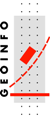
\includegraphics[width=40px]{./images/logo-geoinfo}
\vspace{2.2cm}

\begin{center}
{ \Large
	% Titel
	\textbf{Cloudbasiertes Geodatenmanagement mit Google Fusion Tables: Entwicklung eines Cloud-GIS Prototypen}
	\vspace{1cm}

	% Arbeitstyp / Schule
	\textbf{Studienarbeit}
	\vspace{1cm}

	Abteilung Informatik \\[0.2cm]
	Hochschule für Technik Rapperswil
	\vspace{1cm}

	% Semester
	Frühjahrssemester 2012
}
\end{center}
\vspace{2.3cm}

\begin{tabular}{p{0.19\twocelltabwidth}p{0.81\twocelltabwidth}}
Autoren: & \textbf{Stefan Oderbolz} (\url{soderbol@hsr.ch}) \newline
 \textbf{Jürg Hunziker} (\url{jhunzike@hsr.ch}) \\ 
Betreuer: & \textbf{Prof. Stefan Keller} (\url{sfkeller@hsr.ch}) \\ 
Projektpartner: & \textbf{Marco Lehmann}, GEOINFO AG Herisau, \url{http://www.geoinfo.ch} \\ 
Experte: & \textbf{Prof. Stefan Keller} (\url{sfkeller@hsr.ch}) \\ 
Datum: & \textbf{29. Mai 2012} \\ 
\end{tabular}

\end{titlepage}

% Seitennummerierung mit roemischen Zeichen
\pagenumbering{roman}

% Glossar (muss vor Body inkludiert werden, damit Referenzen funktionieren)
% Glossar
\newglossaryentry{Geocodierung} {
name = Geocodierung,
description = {Bei der Geocodierung wird eine Zeichenkette (Adresse, Namen) einer geografischen Position zugewiesen.}
}


% TODO Liste
\listoftodos

% Impressum & Aenderungsverlauf
\chapter*{Impressum und Revision}
% Titel auch in Kopfzeile anzeigen
\markboth{Impressum und Revision}{Impressum und Revision}

% Impressum
\section*{Impressum}
\begin{longtable}{|l|p{11cm}|}
\hline 
\textbf{Autoren:} & Stefan Oderbolz (\url{soderbol@hsr.ch}) \newline
Jürg Hunziker (\url{jhunzike@hsr.ch}) \\ 
\hline 
\textbf{Dokument erstellt:} & 27.02.2012 \\ 
\hline 
\textbf{Letzte Aktualisierung:} & 29.05.2012 \\ 
\hline 
\end{longtable}

% Aenderungsverlauf
\section*{Änderungsverlauf}

\begin{longtable}{|p{2cm}|p{10cm}|p{3cm}|}
\hline 
\textbf{Datum} & \textbf{Änderungen} & \textbf{Bearbeiter} \\ 
\hline 
27.02.2012 & Dokumententwurf erstellt & Stefan Oderbolz \\ 
\hline 
01.03.2012 & Struktur erstellt & Jürg Hunziker \\ 
\hline 
09.03.2012 & Weitergearbeitet an Einleitung & Jürg Hunziker \\ 
\hline 
05.04.2012 & Mit Dokumentation des Use Cases 1: WorldData begonnen & Jürg Hunziker \\ 
\hline 
06.04.2012 & Benutzerdokumentation erstellt für den Use Cases 1: WorldData & Jürg Hunziker \\ 
\hline 
09.04.2012 & Bildbeschriftungen zu bestehenden Grafiken hinzugefügt & Jürg Hunziker \\ 
% revisions from git
\hline 
\end{longtable} 

% Erklaerung
\chapter*{Erklärung}
% Titel auch in Kopfzeile anzeigen
\markboth{Erklärung}{Erklärung}

Ich erkläre hiermit,
\begin{itemize}
\item dass ich die vorliegende Arbeit selber und ohne fremde Hilfe durchgeführt habe, ausser derjenigen, welche explizit in der Aufgabenstellung erwähnt ist oder mit dem Betreuer schriftlich vereinbart wurde,
\item dass ich sämtliche verwendeten Quellen erwähnt und gemäss gängigen wissenschaftlichen Zitierregeln korrekt angegeben habe.
\end{itemize}

\vspace{3cm}

\begin{tabular}{p{0.5\twocelltabwidth}p{0.5\twocelltabwidth}}
Ort, Datum: & Ort, Datum: \\ 
\end{tabular} 

\vspace{1cm}

\begin{tabular}{p{0.5\twocelltabwidth}p{0.5\twocelltabwidth}}
Name, Unterschrift: & Name, Unterschrift: \\ 
\end{tabular} 

% Abstract
% Titel des Abstracts aendern
\renewcommand{\abstractname}{{\Huge\bfseries Abstract}}

\begin{abstract}
% Seitennummerierung auf Abstract-Seite einschalten
\thispagestyle{plain}

Ziel dieser Arbeit war es das Potentials der Cloud-Datenbank \emph{Goolge Fusion Tables} aufzuzeigen. Dazu wurden zuerst einige Beispiele erstellt, welche die verschiedenen Features der Fusion Table verwenden. Zusätzlich wurden Anwendungsfälle im GIS-Bereich gesucht, welche sich ebenfalls mit Google Fusion Tables umsetzen lassen würden. Diese wurden dann als Prototypen implementiert, um den Aufwand aufzuzeigen, welchen es benötigt, um mit Google Fusion Tables eine GIS-Software zu entwickeln.

Es wurden schlussendlich zwei Anwendungsfälle umgesetzt. Zum einen wurde eine Webapplikation implementiert, die es erlaubt historische Daten von verschiedenen Ländern miteinander zu vergleichen. Das Ziel dabei, war das Anzeigen von grossen Datenmengen auf der Karte.

Als zweiten Anwendungsfall wurde eine mobile WebApp entwickelt, welche es dem Benutzer erlaubt Defekte in seiner Umgebung an die zuständige Behörde zu melden. Google Fusion Table wurde dabei als Datenbank zur Speicherung der gemeldeten Defekte verwendet.
\end{abstract}

% Management Summary / Web-Publikation
\chapter*{Management Summary und Web-Publikation}
% Titel auch in Kopfzeile anzeigen
\markboth{Management Summary und Web-Publikation}{Management Summary und Web-Publikation}

\todo[inline]{Management Summary erstellen}
Das Management Summary soll 2-5 Seiten umfassen sowie eine bis zwei Figuren enthalten. Es richtet sich an den „gebildete Laien“ auf dem Gebiet und beschreibt daher in erster Linie die (neuen und eigenen) Ergebnisse und Resultate der Arbeit. Die Sprache soll knapp, klar und stark untergliedert sein. 
Grundlage für das Management Summary kann der Broschüren-Eintrag sein, den die Abteilung bei Diplomarbeiten jeweils früh verlangt, um eine Broschüre zu drucken. Das Management Summary dient als Vorlage für eine allfällige Web-Publikation.
Das Abstract  und das Management Summary werden - zeitlich gesehen - gegen Schluss der Arbeit geschrieben und bilden zusammen mit den Schlussfolgerungen im technischen Bericht den am häufigsten gelesenen Teil der Arbeit. Diese Dokumente sollen daher am Sorgfältigsten ausgearbeitet sein.
Die folgenden Stichworte sollen die typische Struktur illustrieren, wobei die genaue Ausführung jeweils auf die spezifischen Bedürfnisse und Randbedingungen eines Projekts anzupassen ist. Diese Struktur kann auch für die Präsentation der Arbeit als \emph{Richtschnur} dienen. 
\begin{enumerate}
\item Ausgangslage
	\begin{itemize}
 		\item Warum machen wir das Projekt?
		\item Welche Ziele wurden gesteckt (Kann-Ziele, Muss-Ziele)
		\item Was machen andere / welche ähnlichen Arbeiten gibt es zum Thema?
		\item Vorgehen: Was wurde gemacht? In welchen Teilschritten?
		\item Risiken der Arbeit?
		\item Wer war involviert (Durchführung, Entscheide usw.)?
		\item Was konnte von anderen verwendet werden?
	\end{itemize}
\item Ergebnisse
	\begin{itemize}
 		\item Was ist das Resultat? 
 		\item Bewertung der Resultate, was ist Neuartig an der Arbeit?
 		\item Zielerreichung bezüglich Kann-/Muss-Zielen
 		\item Abweichungen (positiv und negativ) und kurze Begründung dafür (Externe) Kosten der Arbeit?
 		\item Was ist der Nutzen (quantifizierbar/nicht quantifizierbar)?
	\end{itemize}
\item Ausblick
	\begin{itemize}
 		\item Was hat man mit Durchführung des Projekts gelernt?
 		\item Verbleibende Probleme, (zukünftige) Gegenmassnahmen bez. Risiken
 		\item Was würde man anders machen, was ist weiter zu tun
 	\end{itemize}
\end{enumerate}

% Inhaltsverzeichnis
\tableofcontents

% -----------------------------------------
% BODY
% -----------------------------------------
% Neue Seite beginnen um Seitennummerierung zurückzusetzen
\cleardoublepage

% Seitennummerierung mit arabischen Zeichen
\pagenumbering{arabic}

% Einleitung
\part{Einleitung}
\chapter{Einleitung}
\label{einleitung}
Das Ziel dieser Arbeit war das Untersuchen der Möglichkeiten welche die \gls{Cloud}-Datenbank Google Fusion Tables (GFT) bietet. Es sollen einige Prototypen für verschiedenste Anwendungsfälle im \gls{GIS}-Bereich erstellt werden, welche das Potential der Datenbank aufzeigen.

\section{Problemstellung}
Die Aufgabenstellung stammt von der GEOINFO AG\footnote{\url{www.geoinfo.ch}}, welche massgeschneiderte \gls{GIS}-Softwarelösungen für ihre Kunden entwickelt.

Für solche Unternehmen wird es nach und nach schwieriger sich auf dem Markt zu beweisen, da bereits viele cloudbasierte \gls{GIS}-Lösungen sehr günstig oder gar kostenlos erhältlich sind. Durch die zu erstellenden Prototypen soll ersichtlich gemacht werden, welche Anwendungsfälle von bestehenden proprietären \gls{GIS}-Sytemen bereits mit Google Fusion Tables realisierbar wären und welchen Aufwand dies darstellen würde.

\section{Aufgabenstellung}
Im Rahmen dieser Arbeit sollen das Potential aber auch Einschränkungen von Google Fusion Tables für den Einsatzbereich eines öffentlichen Web \gls{GIS} evaluiert werden. Es ist aufzuzeigen, welche der typischen Anwendungsfälle, wie sie in aktuellen Web \gls{GIS} Lösungen\footnote{z.B. \url{www.geoportal.ch} oder \url{www.stadtplan.stadt-zuerich.ch}} implementiert sind, auf Basis von Google Fusion Tables und Google Maps realisiert werden könnten. Eine Auswahl dieser Grundfunktionen ist anhand eines Prototypen zu implementieren. Die Zielgruppe sind demnach \gls{GIS}-Sachbearbeiter.

\section{Ziele}
In der Aufgabenstellung der Arbeit wurden folgende Ziele definiert:
\begin{itemize}
\item Evaluation von Google Fusion Tables in Kombination mit Google Maps u.a. mit Blick auf deren Funktionalität, Anwendbarkeit, Zuverlässigkeit und Performance
\item Entwurf und Dokumentation einer \gls{GIS}-Architektur, welche einerseits \gls{Cloud} Services (am Beispiel von Fusion Talbes) andererseits die Geodaten- und Serviceinfrastruktur einer Organisation integriert oder migriert.
\item Analyse verschiedener Use Cases wobei einer davon als Prototyp einer Webapplikation (voll) implementiert werden soll. 
\item Implementierung und Bewertung von verschiedenen cloudbasierten \gls{GIS}-Prototypen unter Verwendung der Google Fusion Tables \gls{API}
\begin{itemize}
	\item Prototyp(en) aus Use Case-Evaluation (oben). Dabei sollen v.a. auch die Geometrietypen Linestring und Polygon berücksichtigt werden.
	\item Prototyp einer Datenerfassung/Verwaltung am Beispiel eines Point-of-Interest (POI) Layers mit grossen Datenmengen
\end{itemize}
\item Prototyping für zukünftige (\gls{GIS}-) Kollaborationsplattformen. Es soll aufgezeigt werden, wie sich bestehende Konzepte\footnote{z.B. \url{www.mysg.ch/locations} oder \url{http://ch.tilllate.com/de/locations})} verbessern lassen oder weiterentwickeln könnten.
\end{itemize}

\section{Rahmenbedingung}
\begin{itemize}
\item Es gelten die Rahmenbedingungen, Vorgaben und Termine der HSR
\item Die Projektabwicklung orientiert sich an einer iterativen, agilen Vorgehensweise. Als Vorgabe dient dabei Scrum, wobei bedingt durch das kleine Projektteam gewisse Vereinfachungen vorgenommen werden. Meilensteine werden bezüglich Termin und Inhalt mit dem verantwortlichen Dozenten und dem Projektpartner vereinbart.
\item Die Kommunikation in der Projektgruppe, in der Dokumentation und an den Präsentationen erfolgt in Deutsch.
\item Eine Prototypen-Website ist in HTML/JavaScript zu implementieren und sollte auf verschiedenen Plattformen lauffähig sein.
\end{itemize}

\section{Vorgehen}
Die Arbeit umfasst zwei Themenbereiche: Einen theoretischen Teil in dem untersucht wird, inwiefern Google Fusion Tables eine Konkurrenz für bestehende proprietäre \gls{GIS}-Lösungen darstellt. Als zweiten Teil sollen verschiedene Anwendungsfälle mit Google Fusion Tables als Prototypen nachgebaut werden, wobei einer davon als mobile Webapplikation ausprogrammiert werden soll.

\subsection{Potential von Google Fusion Tables}
Es soll aufgezeigt werden, inwiefern sich Anwendungsfälle aus bestehenden \gls{GIS}-Lösungen mit Google Fusion Tables abbilden lassen.

Zu diesem Zweck sollen Use Cases erarbeitet werden, welche ein möglichst breites Spektrum abbilden können. Wichtige Themen sind dabei das Verwaltung von grösseren Datenmengen, die Verwaltung von Daten aus verschiedenen Quellen und die Kollaboration bei der Bearbeitung der Daten.

Dabei soll aufgezeigt werden, wie Daten nach Google Fusion Tables migriert werden können und anschliessend eine Weiterverarbeitung erfolgen kann. Da sich die Datenstrukturen von bestehenden Lösungen stark unterscheiden können, ist es nicht das Ziel eine Schritt-für-Schritt Anleitung zu erstellen. Primär geht es darum die Möglichkeiten aufzuzeigen.

Durch die theoretische und praktische Auseinandersetzung mit Google Fusion Tables soll das gegenwärtige Potential dieses Dienstes abgeschätzt werden. Diese Erkenntnis soll \gls{GIS}-Lösungsprovidern einen Überblick verschaffen, inwiefern Google Fusion Tables bereits eingesetzt werden kann bzw. wo dessen Stärken und Schwächen liegen.

\subsection{Erstellung von Prototypen}
Der theoretische Teil soll dann schliesslich durch verschiedene Prototypen belegt werden. Es soll versucht werden mehrere Standard-Anwendungsfälle im \gls{GIS}-Bereich mittels Google Fusion Tables zu realisieren. Diese Prototypen sollen in Form von Webapplikationen entwickelt werden, um eine grösstmögliche Plattformunabhängigkeit zu erreichen.

Ein Anwendungsfall soll zusätzlich als vollwertige Webapplikation für Mobilgeräte ausprogrammiert werden.

\section{Aufbau der Arbeit}
Die Arbeit ist in drei Teile gegliedert. Zuerst kommt eine theoretische Einführung ins Thema mit einer Abschätzung des Potentials von Google Fusion Tables (siehe Kapitel \ref{einleitung} und \ref{einfuehrung}) und unserer Infrastruktur (siehe Kapitel \ref{infrastruktur}), im zweiten Teil gehts es dann um die erstellten Arbeitsresultate (siehe Kapitel \ref{beispielapplikationen}, \ref{worlddata}, \ref{fixmystreet} und \ref{converter-build}) und schliesslich im letzten Teil um das Projektmanagement (siehe Kapitel \ref{projektmanagement}).

Wir haben während dem Semester Sitzungen mit unserem Betreuer durchgeführt und auch unseren Auftraggeber zweimal getroffen. Dadurch haben wir regelmässig Feedback zu unserem Arbeitsfortschritt erhalten und konnten unseren Stand präsentieren.

Neben diesem Dokument umfasst diese Arbeit zahlreiche Beispielanwendungen und zwei Webapplikationen, welche im Internet verfügbar sind. Der dazugehörige Source Code ist ebenfalls frei im Internet zugänglich sowie auf der beigelegten CD zu finden.

\begin{longtable}{|l|l|}
\hline 
\textbf{Arbeitsresultat} & \textbf{URL} \\ 
\hline 
Übersichtsseite & \url{http://gft.rdmr.ch} \\ 
\hline 
WorldData Use Case & \url{http://worlddata.rdmr.ch} \\ 
\hline 
FixMyStreet Use Case & \url{http://fixmystreet.rdmr.ch} \\ 
\hline 
Converter-Build & \url{http://jenkins.rdmr.ch:8080/job/Convert-GIS-files/} \\ 
\hline 
Repsitory & \url{https://github.com/odi86/GFTPrototype} \\ 
\hline 
\caption{Übersicht aller Arbeitsresultate}
\label{arbeitsresultate}
\end{longtable} 

\section{Stand der Technik}
Diese Arbeit beschäftigt sich mit sogenannten \gls{Cloud}-Datenbanken, mit einem Fokus auf ortsbezogene Daten. Wichtig sind dabei die verschiedenen Möglichkeiten zur Visualisierung von Daten. Dieser Abschnitt erklärt die zugehörigen Konzepte und Produkte.

\subsection{Software-as-a-Service (SaaS) / Infrastructure-as-a-Service (IaaS)}
Der Begriff \emph{Software-as-a-Service} (\gls{SaaS}) hat sich in den letzten Jahren etabliert und bezeichnet die Dienstleistung eine Software nicht nur für einen Kunden zu entwickeln, sondern auch gleich deren Betrieb zu übernehmen. Diese gesamthafte Dienstleistung wird dann dem Kunden angeboten, so dass dieser keine eigene Infrastruktur betreiben muss. Die \gls{Cloud} ist die logische  Erweiterung dieses Konzepts, dabei wird der angebotene Dienst transparent auf mehreren Umgebungen und an verschiedenen Lokationen angeboten. Dies soll zum einen eine hohe Erreichbarkeit gewährleisten und zum anderen die Skalierbarkeit erleichtern.\cite{cloud}

Bei Google Fusion Tables handelt es sich genau genommen um eine Infrastructure-as-a-Service (IaaS) Dienstleitung\footnote{Einordnung gemäss \url{https://www.e-education.psu.edu/cloudGIS/node/91}}), da lediglich die Speicherung der Daten ausgelagert ist. Grundsätzlich würde Google aber das ganze Portfolio anbieten (Webserver,  Software etc.).

\subsection{Datenbank in der Cloud}
\gls{Cloud}-Datenbanken wie Google Fusion Tables schaffen das Problem der Erreichbarkeit ab. Sie sind dezentral in der \gls{Cloud} gespeichert und lassen sich  einfach vertikal skalieren. Dies vereinfacht den Zugang zu den Daten und ermöglicht es diese mit anderen Personen zu teilen. Dank der bereitgestellten Infrastruktur kann sich ein Anwender der Datenbank auf das wesentliche konzentrieren: die Daten in geeigneter Form abzulegen und auszulesen.

\subsection{Produkte}
Neben der in dieser Arbeit beschriebenen Google Fusion Tables (siehe Kapitel \ref{einfuehrung}) gilt es vor allem noch das Produkt CartoDB zu erwähnen. CartoDB\footnote{\url{http://cartodb.com/}} basiert auf PostGIS\footnote{\url{http://postgis.refractions.net/}}, einer PostgreSQL-Erweiterung für geografische Daten. Das Projekt wurde während unserer Arbeit, am 3. April 2012, veröffentlicht\footnote{Welcome to CartoDB 1.0 \url{http://blog.cartodb.com/post/20403296927/welcome-to-cartodb-1-0}}. Das Projekt ist Open-Source und lässt sich somit komplett in einer eigenen Umgebung installieren\footnote{Repository mit Installationsanleitung: \url{https://github.com/Vizzuality/cartodb}}.

Daneben bietet CartoDB aber wie Google auch die Möglichkeit den Dienst von ihnen zu beziehen (\gls{SaaS}). Obwohl  die Konzepte sehr verschieden sind, sind die beiden Produkte durchaus miteinander vergleichbar\footnote{CartoDB hat einen Vergleich zwischen ihrem Produkt und Google Fusion Tables veröffentlicht. Auch wenn der Artikel stark einseitig gefärbt ist, zeigt er doch ein paar interessante Unterschiede auf: \url{http://blog.cartodb.com/post/21264086445/comparing-fusion-tables-to-open-source-cartodb}}.

\section{Vision/Umsetzungskonzept}
Um das Potential von Google Fusion Tables bewerten zu können, mussten wir uns zuerst mit dem Dienst vertraut machen. Die Idee war es, verschiedene Prototypen zu erstellen, welche jeweils verschiedene Aspekte des Produktes aufzeigen. Die Prototypen sollten sich dabei an gängige Aufgabenstellungen aus dem \gls{GIS}-Bereich anlehnen.

Neben dem \gls{GIS}-Aspekt war es uns wichtig unabhängige Lösungen zu bauen welche auf möglichst vielen Plattformen laufen. Aus diesem Grund haben wir uns einerseits für webbasierte Applikationen entschieden, andererseits in möglichst allen Bereichen mit \gls{Cloud}-gestützten Diensten gearbeitet. Der Serveranteil sollte dabei so gering wie möglich sein, um keine unnötigen Abhängigkeiten und Hürden zu schaffen.

Da wir der festen Überzeugung sind, dass mobile Applikationen immer wichtiger werden, haben wir Wert darauf gelegt, dass die Prototypen mobile-fähig sind. 

\section{Resultate der Arbeit}
Wir haben das gesteckte Ziel, das Potential von Google Fusion Tables abzuschätzen, sehr gut erreicht. Unser schrittweises Vorgehen hat sich ausbezahlt. Wir konnten zu Beginn die Theorie und den Praxiseinsatz sehr rasch lernen, in dem wir zahlreiche Beispielapplikationen entwickelt haben. So konnten wir uns langsam einen Überblick über die Möglichkeiten und Limitation von GFT machen.

Während der Arbeit hat es sich dann ergeben, dass wir sogenannte \emph{Trusted Tester} für das neue \gls{API} von Google wurden. Dort konnten wir neuen Features ausprobieren und standen in direktem Kontakt mit den Fusion Tables Entwicklern (siehe Abschnitt \ref{austausch-mit-google}). Gerade mit dem neuen \gls{API} haben wir komplettes Neuland betreten. Die von uns geschriebene JavaScript Library bietet einen einfachen Zugang zu diesem \gls{API}.

Später haben wir uns dann auf die Umsetzung der Use Cases konzentriert. Die Idee dabei war es, möglichst realistische Szenarien zu finden und dann eine mögliche Lösung mit Google Fusion Tables aufzuzeigen. Beim \emph{WorldData} Use Case lag dabei das Gewicht auf dem Importieren und Zusammenführen von Daten aus verschiedenen Quellen sowie der Handhabung von grösseren Datenmengen (siehe Kapitel \ref{worlddata}). Beim zweiten Use Case \emph{FixMyStreet} stand eher die Kollaboration, der Live-Gedanke und die Nutzung von GFT als Applikations-Datenbank im Vordergrund (siehe Kapitel \ref{fixmystreet}).

Ursprünglich wollten wir 3 Use Cases umsetzen, wir haben uns dann aber im Verlauf der Arbeit und in Absprache mit unserem Betreuer und dem Industriepartner dazu entschieden, nur 2 Use Cases umzusetzen. Dies vor allem aus zeitlichen Gründen. Dadurch konnten wir einen der beiden Use Cases vertiefen und daraus einen vollwertigen Web-App Prototypen bauen.

Zusätzlich haben wir ein Tool bereitgestellt mit dem sich zum einen Geodaten in andere Formate konvertieren lassen und zum anderen direkt Dateien als Tabellen in Google Fusion Tables importieren lassen (siehe Kapitel \ref{converter-build}).

\section{Schlussfolgerungen und Ausblick}
Das Fazit unserer Arbeit fällt gemischt aus. Zum einen bietet Google Fusion Tables einen kostenlosen Dienst an, welcher für kleinere Anwendungen genügend bietet sowohl als Datenbank-Backend wie auch als Speicherort für Daten eines Benutzers. Das SQL \gls{API} hingegen ist an einigen Stellen noch unvollständig und lässt sich noch nicht mit dem einer vollwertigen Datenbank vergleichen.

Die Handhabung davon ist dagegen sehr einfach und entspricht meistens den Erwartungen. Die Dokumentation ist sehr gut und ausführlich. Falls doch Fragen auftauchen gibt es eine aktive Community, an die man sich wenden kann. 

Ein grosses Plus ist die einfache Bedienung und die zahlreichen Visualisierungsmöglichkeiten, welche Google bereits anbietet. Durch die Integration in Google Maps können Daten sehr einfach auf einer Karte dargestellt werden.

Zum anderen gibt es aber einige harte Limiten, welche einen daran hindern grössere Applikationen damit zu bauen. Die Limite beispielsweise, welche vorgibt, dass jeweils nur die ersten 100'000 Datensätze einer Tabelle als Result eines Queries geliefert werden, kann für grössere Datensammlungen zu einem Problem werden. Auch die Anzahl gleichzeitiger Zugriffe ist limitiert, sofern man dafür nicht extra bezahlen möchte.

Wenn man die Features ansieht, merkt man schnell, dass ein Typ Use Case unterstützt wird, jedoch nicht viel mehr. Es gibt zwar die Möglichkeit über Merged Tables einen \inlinecode{LEFT OUTER JOIN} von 2 Tabellen hinzubekommen, jedoch wäre die normale SQL \inlinecode{JOIN}-Syntax sehr wünschenswert, da sich damit beliebige Abfragen realisieren lassen. 

Die \gls{OAuth} Dokumentation ist zwar für den Normalfall (Zugriff auf Tabellen eines Benutzers) sehr gut dokumentiert. Das neue \emph{Service Account}-Modell findet aber noch fast keine Erwähnung. Die Handhabung ist etwas sperrig, schlussendlich aber doch machbar. Leider sind momentan die Berechtigungen nur sehr grob einstellbar. So gibt es lediglich einen \gls{OAuth}-Scope, und dieser ermöglicht alle Schreiboperationen auf einem Account. Für einige Situationen wäre es wünschenswert gewisse SQL-Befehle (z.B. \inlinecode{DELETE}) zu verbieten.

Das Web-GUI der Google Fusion Tables lässt ebenfalls noch einige Wünsche offen. Zum einen läuft es nicht sehr stabil und zum anderen ist die Bedienung nicht wirklich intuitiv. Das neue, sogenannte \emph{experimental UI}, hat schon einige Verbesserungen gebracht, es fehlen aber einige Funktionen, welches das "`alte"' UI bot. So lassen sich zum Beispiel keine Views mit einer \inlinecode{WHERE}-Klausel über das Web-GUI definieren. 

Das neue \gls{API} sieht sehr vielversprechend aus. Die Entwickler bei Google sind grundsätzlich offen für Anregungen, Kritik oder Feature Requests. Es bleibt abzuwarten, wie sich GFT und das Konkurrenzprodukt CartoDB zukünftig positionieren werden.

% Projektdokumentation
\part{Projektdokumentation}
\chapter{Projektdokumentation}

\section{Resultate der Beispiele}

\subsection{SQL API}
Das SQL API bietet eine REST-Schnittstelle mit welcher man mit SQL-ähnlichen Befehlen Daten aus Google Fusion Tables abfragen oder verändern kann. Sie verfügt bereits über eine grosse Palette an möglichen Befehlen.

\begin{tabular}{|l|l|}
\hline 
Befehl & Beschreibung \\ 
\hline 
SHOW TABLES & Abfrage aller Tabellen des angemeldeten Benutzers \\ 
\hline 
DESCRIBE & Bezeichnung und Datentypen aller Spalten in einer Tabelle \\ 
\hline 
CREATE TABLE & Erstellen einer neuen Tabelle \\ 
\hline 
CREATE VIEW & Erstellen einer View auf Grundlage einer bestehenden Tabelle \\ 
\hline 
SELECT & Selektieren von Daten einer Tabelle \\ 
\hline 
INSERT & Neue Zeile zu einer Tabelle hinzufügen \\ 
\hline 
UPDATE & Daten in einer Tabelle verändern \\ 
\hline 
DELETE & Daten aus einer Tabelle löschen \\ 
\hline 
DROP TABLE & Löschen einer Tabelle \\ 
\hline 
\end{tabular}

\subsubsection{Client Libraries}
Google bietet zum API bereits auch Client Libraries in den Sprachen PHP und Phyton an. Da unserer Applikation aber möglichst nur in Javascript implementiert werden soll erstellten wir uns eine Javascript Library zur Verwendung des SQL APIs.

Durch die Same origin policy\footnote{Die Same-Origin-Policy (SOP) ist ein Sicherheitskonzept, das es JavaScript und ActionScript nur dann erlaubt, auf Objekte einer anderen Webseite zuzugreifen, wenn sie aus derselben Quelle (Origin) stammen.\cite{sop} }, welche es uns daran hinderte AJAX-Requests direkt auf das Google API abzusetzen, mussten wir zuerst nach Lösungen für dieses Problem suchen. Wir wollten es verhindern einen PHP-Server dazwischen zu schalten, welcher uns die Abfragen abnimmt.

So fanden wir in den Google Groups ein inoffizielles JSONP API, welches es erlaubt AJAX-Requests auch über die eigene Domäne hinweg zu senden.

\subsubsection{Spatial-Queries}
Das SQL API bietet bereits eine Reihe von speziellen ortsabhängigen Abfrage-Möglichkeiten.
\begin{tabular}{|l|l|}
\hline 
Spatial condition & Beschreibung \\ 
\hline 
ST\_INTERSECTS\(<location\_column>, <geometry>\) & Liefert alle Zeilen zurück, welche sich innerhalb der definierten Geometrie befinden. \\ 
\hline 
ST\_DISTANCE\(<location\_column>, <coordinate>\) & • \\ 
\hline 
CIRCLE & • \\ 
\hline 
NEAR & • \\ 
\hline 
POLYGON & • \\ 
\hline 
RECTANGLE & • \\ 
\hline 
\end{tabular} 

\subsection{Geocodierung}
Ein grosser Vorteil der Google Fusion Tables ist die automatische 
\gls{Geocodierung} von Standortdaten. Sobald eine neue Zeile zu einer Tabelle hinzugefügt wird, werden alle Zellen vom Typ \emph{Location} einem eindeutigen Standort auf der Karte zugewiesen. Ist dies nicht möglich, da beispielsweise eine Adresse in mehreren Orten vorkommen kann, bleibt die Zelle gelb hinterlegt.
 
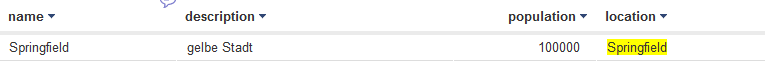
\includegraphics[scale=0.75]{images/geocoding_failed.png}

Diese geocodierten Standorte werden in der Tabelle hinterlegt sind aber mit den SQL API nicht selektierbar. Man müsste also für jede Zeile die man als Resultat erhält die Geocodierung selbst vornehmen, was sich negativ auf die Ladezeit der Karte auswirkt.
Es gibt verschiedene Dienste, welche eine solche Geocodierung von Standortdaten anbieten. Die meisten davon haben aber eine Begrenzung der möglichen Anfragen pro Tag.

\begin{tabular}{|l|l|l|}
\hline 
Anbieter & Anfragen pro Tag & URL \\ 
\hline 
Google Maps Geocoding API & 2500 & https://developers.google.com/maps/documentation/geocoding/?hl=de \\ 
\hline 
Yahoo! PlaceFinder API & 50000 & http://developer.yahoo.com/geo/placefinder/ \\ 
\hline 
MapQuest Geocoding API & keine Begrenzung & http://developer.mapquest.com/web/products/dev-services/geocoding-ws \\ 
\hline 
\end{tabular} 

Wie man sieht erreicht man mit diesen Diensten beim Arbeiten mit grossen Datenmengen schnell die Grenzen.

\subsection{Google Maps API FusionTableLayer}
Google bietet von Haus aus aber bereits eine Fusion Table-Integration im Google Maps API V3 an. Damit ist es möglich Tabellen als eigenständige Layer direkt auf der Karte darzustellen.
Die Möglichkeiten dieser Layer sind noch stark eingeschränkt aber die grundlegenden Funktionalitäten für das Arbeiten mit Geodaten sind bereits vorhanden.

So ist es möglich Abfragen mit WHERE-Conditions einzuschränken oder die Stile des Layers selbst zu bestimmen. Man kann beispielsweise Flächen mit Zeckengebieten je nach Intensität des Befalls anders einfärben.

Ein mächtiges Feature ist zudem die Möglichkeit die Daten der Tabelle direkt als Heatmap darzustellen.

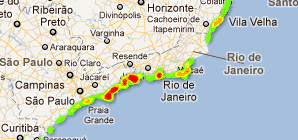
\includegraphics{images/gmap_fusiontableslayer_heatmap.png}

\subsubsection{Vorteil}
Der grösste Vorteil der Fusion Table-Ebenen findet man aber eher darin, dass die Geocodierung der Standort-Daten direkt aus der Tabelle gelesen wird und nicht manuell abgefragt werden muss. Dadurch kann die Ebene komplett auf den Servern von Google aufbereitet werden. Der Client muss die erhaltenen Daten lediglich noch darstellen. Der Vorteil davon wird durch das folgende Diagramm schnell ersichtlich.

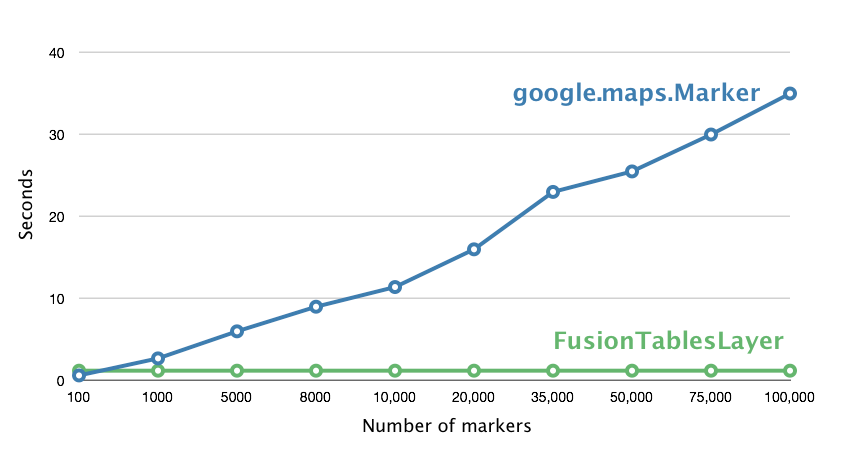
\includegraphics[scale=0.5]{images/gmap_fusiontableslayer_vs_markers.png}

Die Zeit für das Rendering der Karte bleibt demnach beim arbeiten mit Fusion Table-Ebenen konstant und somit unabhängig von der Anzahl Markierungen, welche gesetzt werden müssen. Der Rechenaufwand für das Erstellen der Javascript Marker-Objekte wird direkt von den Google Servern übernommen und das Resultat als Bild zum Client gesendet. Daraus resultiert die konstante Zeit, welche für die Anfrage zum Server und für das Senden der Antwort zum Client verwendet wird.

\subsubsection{Nachteil}
Ein grosser Nachteil dieser Fusion Table-Ebenen besteht aber darin, dass die verwendeten Fusion Tables als  \emph{öffentlich} markiert sein müssen. Sprich jeder kann die Tabellen anzeigen oder auslesen. Es ist also nicht möglich eine Tabelle mit sensiblen Daten als Fusion Table-Ebene darzustellen.

Von Google wird zur Lösung dieses Problems aber folgendes Vorgehen vorgeschlagen: Man kann für Tabellen mit sensiblen Inhalten eine View erstellen, welche lediglich die öffentlichen Spalten und Zeilen selektiert. Diese View könnte man dann als \emph{öffentlich} markieren und in einer Fusion Table-Ebene verwenden.

Es bleibt die Frage offen, wie es möglich ist sensible Daten trotzdem in eine Ebene einzubringen.

\section{Google Fusion Table Javascript Library (gftlib-js)}
Die Google Fusion Table Javascript Library vereinfacht die Kommunikation mit dem Google Fusion Table SQL API. Sie hilft dabei SQL-Queries zu erstellen und per AJAX an das API zu versenden.

Zur Erstellung der AJAX-Requests werden die \$.get()- und \$.post()-Helpermethoden der jQuery Library in der Version 1.7.1 (Minified) verwendet.

\subsection{Methoden}
\begin{tabular}{|l|l|l|}
\hline 
Methode & Beschreibung & Parameter \\ 
\hline 
execSql(callback, query) & Führt einen SQL-Befehl & callback (Funktion): Callback-Methode welche nach Beendigung der Methode aufgerufen wird. query (String): SQL-Query \\ 
\hline 
execSelect(callback, options) & Führt einen SQL-Abfrage aus & callback (Funktion): Callback-Methode welche nach Beendigung der Methode aufgerufen wird. query (String): SQL-Query \\ 
\hline 
convertToObject(gftData) & Konvertiert das Resultat einer Abfrage in sprechende Objekte & • \\ 
\hline 
\end{tabular} 



\section*{Beispiel für Codeschnippsel}
\lstset{language=HTML}
\begin{lstlisting}
<h1>test</h1>
<!-- comment -->
\end{lstlisting}

\section{Überblick}

\section{Vision}

\section{Anforderungsspezifikation}

\section{Analyse}

\section{Design}

\section{Implementation}

\section{Test}

\section{Resultate}

\section{Weiterentwicklung}

\section{Benutzerdokumentation}


% Projektmanagement
\part{Projektmanagement}
\chapter{Projektmanagement}

\section{Allgemeines}

\section{Projektmanagement}

\section{Projektmonitoring}


% -----------------------------------------
% FOOT
% -----------------------------------------
\part{Anhänge}

% Glossar
\printglossary[style=altlist,title=Glossar,toctitle=Glossar]

% Literaturverzeichnis
\bibliographystyle{plainurl}
\bibliography{foot/literatur}

% Abbildungsverzeichnis
\listoffigures

\end{document}